\documentclass[international_finance_p2.tex]{subfiles}

\begin{document}
\setbeamercovered{transparent}
\section{Absolute Purchasing Power Parity}
\begin{frame}{Absolute Purchasing Power Parity (PPP)}
\begin{align}
E=\frac{P}{P^F}
\end{align}
where 

$E$ is the spot exchange rate (domestic currency units per foreign unit);

$P$ the domestic price index;

$P^F$ the foreign price index.

$P$ and $P^F$ may be thought of as consumer price indexes or producer price indexes.

Absolute PPP indicates that the exchange rate between any two currencies is equal to the ratio of their price indexes.
\end{frame}
\subsection{The Big Mac Index}
\begin{frame}
\begin{block}{The Big Mac Index}
\quad is published by The Economist (http://www.economist.com) as an informal way of measuring the purchasing power parity (PPP) between two currencies and provides a test of the extent to which market exchange rates result in goods costing the same in different countries.
\end{block}
\end{frame}
\begin{frame}{The Big Mac index}
\begin{columns}
\begin{column}{0.5\textwidth}
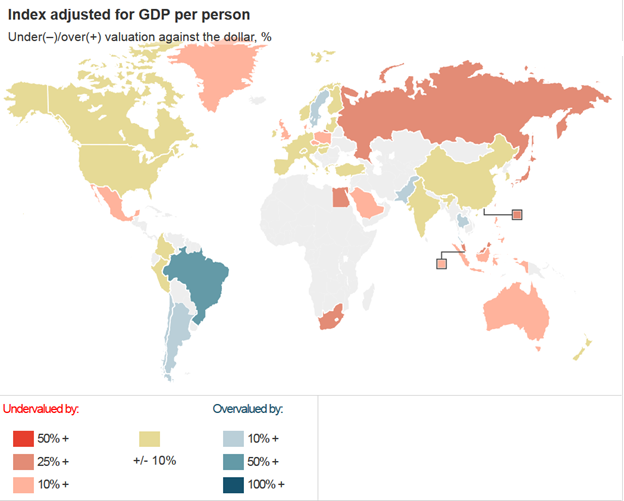
\includegraphics[scale=0.5]{img/bigmac}
\end{column}
\begin{column}{0.4\textwidth}

Sources: McDonald`s, The Economist. 2016.
\end{column}
\end{columns}
\end{frame}

\subsection{Relative Purchasing Power Parity}
\begin{frame}{Relative Purchasing Power Parity}
\begin{align}
\Delta E=\Delta P- \Delta P^F,
\end{align}
where 
$\Delta E$ is equal to the percentage change in the domestic price level ($\Delta P$) minus the percentage change in the foreign price level ($\Delta P^F$).

Absolute PPP states that the exchange rate is equal to the ratio of the price indexes, relative PPP deals with percentage changes in these variables.

If absolute PPP holds, then relative PPP will also hold. But if absolute PPP does not hold, relative PPP still may. This is so because the level of $E$ may not equal $\frac{P}{P^F}$, but the change in $E$ could still equal the inflation differential.
\end{frame}

\subsection{Overvalued and Undervalued Currencies}
\begin{frame}{Overvalued and Undervalued Currencies}
\begin{block}{Overvalued and Undervalued Currencies definition}
\quad If, over time, foreign price index rises faster than domestic price index, then we would expect spot exchange rate, the domestic currency price of the foreign currency, to fall. If E does not fall by the amount suggested by the lower $\frac{P}{P^F}$, then the domestic currency is undervalued or (the same thing) that the foreign currency is overvalued.
\end{block}
\end{frame}
\begin{frame}{The implied PPP exchange rate}
\begin{itemize}[<+->]
\item
The implied PPP exchange rate measures the values the exchange rate would take if the percentage change in the exchange rate equaled the inflation differential between two countries. 
\item
If the spot exchange rate is greater than the implied PPP exchange rate than the currency is supposed to be overvalued. Otherwise, the currency would be undervalued.
\end{itemize}
\end{frame}

\subsection{Real Exchange Rates}
\begin{frame}{Real Exchange Rates}
\begin{itemize}[<+->]
\item
The real interest rate is the rate of interest is expected rate to receive after adjustment for inflation.
\item
The real exchange rate is the purchasing power of a currency relative to another at current exchange rates and prices.
\end{itemize}
\end{frame}

\end{document}